\section{Model}
Here a model is presented using the conventions shown in \autoref{fig:system} and assuming zero friction in the system.

The energy method is applied to find the dynamic equations using generalized coordinates, $x$ and $\theta$, as defined in \autoref{fig:system}. The kinetic energy $T$ is given by,
%
\begin{flalign}
  T &= \frac{1}{2} M \dot{x}^2 + \frac{1}{2} m (\dot{x} + l \dot{\theta} \cos \theta )^2 + \frac{1}{2} m (-l \dot{\theta} \sin \theta )^2  & \nonumber \\ % \unit{N \cdot m}\\
  T &= \frac{1}{2} (M+m) \dot{x}^2 + m \dot{x} l \dot{\theta} \cos \theta + \frac{1}{2} m l^2 \dot{\theta}^2 \ \ \ . & \unit{N \cdot m}
  \label{eq:kineticEnergy}
\end{flalign}
%
\begin{where}
  \va{ T                 }{is the kinetic energy}                      {N \cdot m}
  \va{ M                 }{is the mass of the cart}                    {kg}
  \va{ \dot{x}           }{is the velocity of the cart}                {m \cdot s^{-1}}
  \va{ m                 }{is the mass of the pendulum}                {kg}
  \va{ l                 }{is the length of the pendulum}              {m}
  \va{ \theta            }{is the angle of the pendulum}               {rad}
  \va{ \dot{\theta}      }{is the angular velocity of the}             {rad \cdot s^{-1}}
\end{where}

The potential energy is given by,
%
\begin{flalign}
  V &= M g l \cos \theta \ \ \ . & \unit{N \cdot m}
  \label{eq:potentialEnergy}
\end{flalign}
%
\begin{where}
  \va{ V                 }{is the potential energy}                    {N \cdot m}
  \va{ g                 }{is the gravitational acceleration}          {m \cdot s^{-2}}
\end{where}

By \autoref{eq:kineticEnergy} and \autoref{eq:potentialEnergy} the Lagrangian becomes,
%
\begin{flalign}
  \cal{L} &= T - V & \nonumber \\ 
  \cal{L} &= \frac{1}{2} (M+m) \dot{x}^2 + m \dot{x} l \dot{\theta} \cos \theta + \frac{1}{2} m l^2 \dot{\theta}^2 - M g l \cos \theta \ \ \ . & \unit{N \cdot m}
  \label{eq:lagrangian}
\end{flalign}
%
\begin{where}
  \va{ \cal{L}           }{is the Lagrangian}                          {N \cdot m}
\end{where}

From the energy method we find the dynamic equations corresponding to each of the generalized coordinates, $\theta$ and $x$, by,
%
\begin{flalign}
  \frac{d}{dt} \left( \frac{\partial \cal{L}}{\partial \dot{\theta}} \right) - \frac{\partial \cal{L}}{\partial \theta} &=  0  & \\ %\unit{N \cdot m}  \\
  \frac{d}{dt} \left( \frac{\partial \cal{L}}{\partial \dot{x}} \right) - \frac{\partial \cal{L}}{\partial x} &=  f  \ \ \ . & %\unit{N \cdot m}
  \label{eq:energyMethod}
\end{flalign}
%
\begin{where}
  \va{ f          }{is the actuation force, see \autoref{fig:system}}             {N \cdot m}
\end{where}

Inserting the Lagrangian and reducing the expressions finally yields the dynamic equations,
%
\begin{flalign}
  m l \cos \theta \ddot{x} + m l^2 \ddot{\theta} - m l g \sin \theta &=  0  & %\unit{N \cdot m}  \\
  \label{eq:dynamicEquation1} \\
  (M+m) \ddot{x} + m l \cos \theta \ddot{\theta} - m l \sin \theta \dot{\theta}^2 &= f  \ \ \ . & %\unit{N \cdot m}
  \label{eq:dynamicEquation2}
\end{flalign}

A block diagram is derived in \autoref{fig:blockDiagram} from \autoref{eq:dynamicEquation1} and \autoref{eq:dynamicEquation2}.

\begin{figure}[H]
  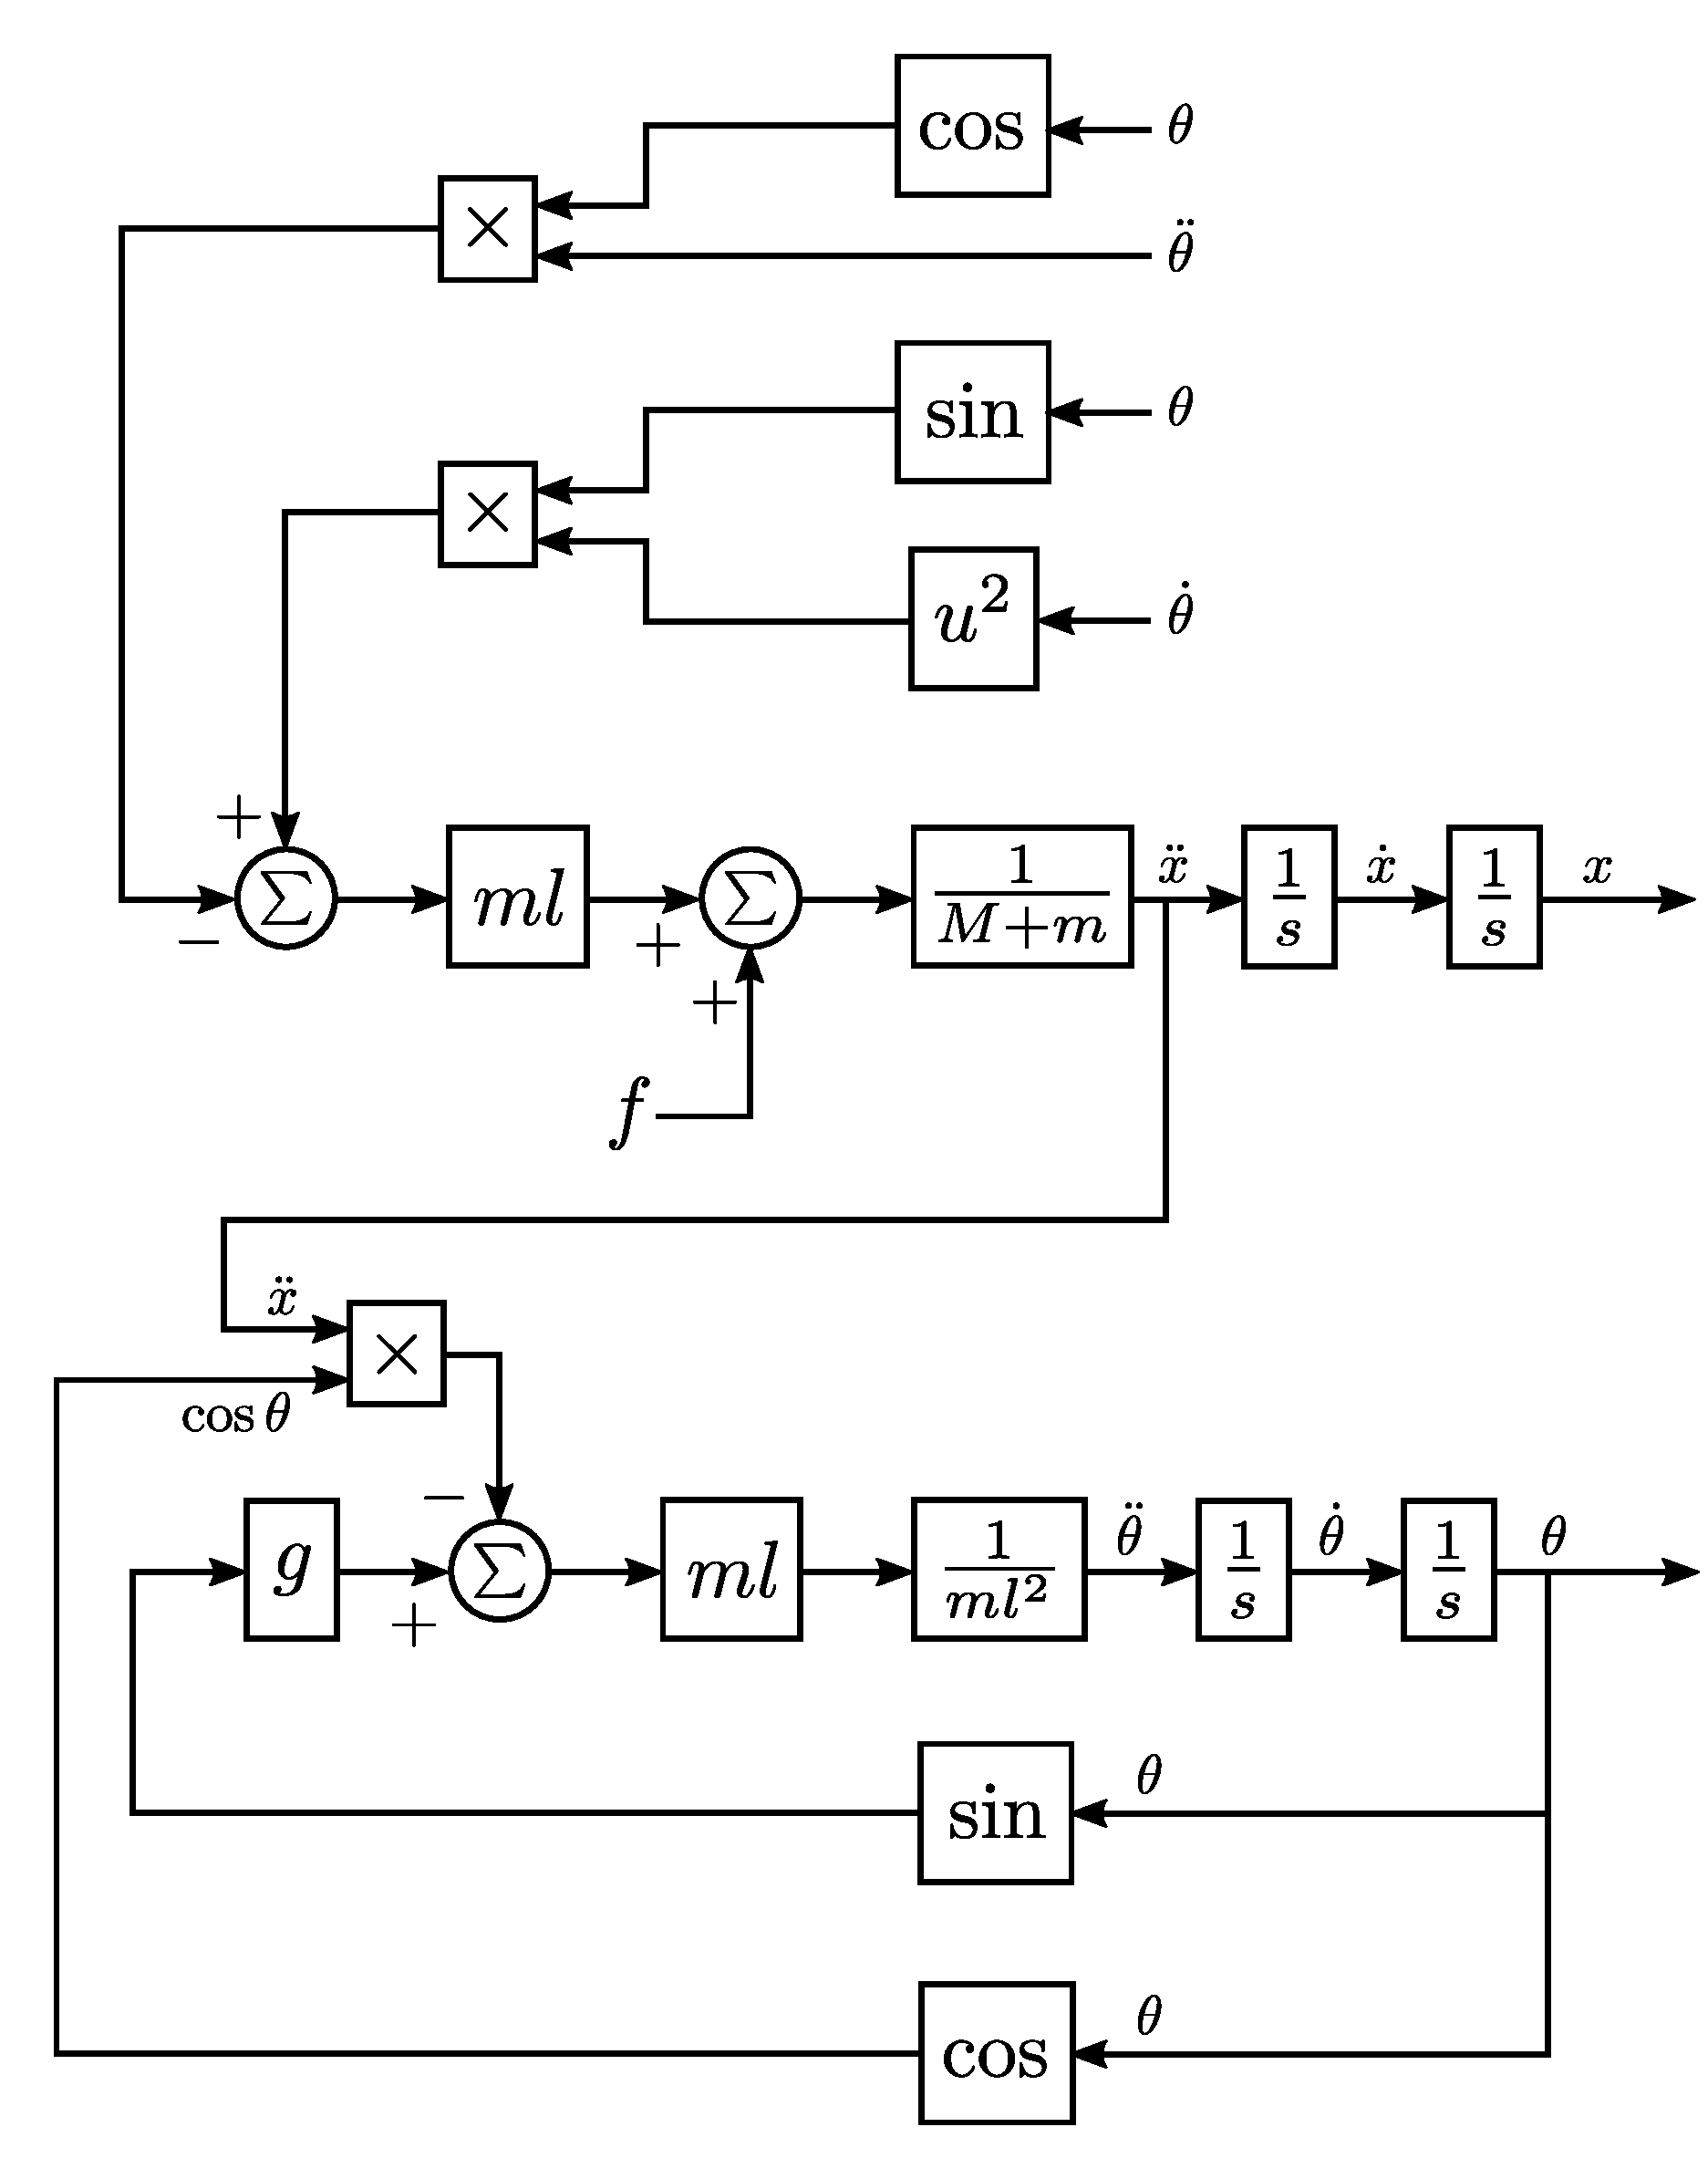
\includegraphics[width=.5\textwidth]{figures/blockDiagram}
  \caption{A block diagram derived from the dynamic equations, later used for simulation. The four signals in the top, $\theta$, $\dot{\theta}$ and $\ddot{\theta}$, are drawn without explicit connection only to keep the figure clear.}
  \label{fig:blockDiagram}
\end{figure}

This is implemented in Matlab Simulink to be able to simulate the system. A graphical layer, including the obstacles, is added to the simulation to show the system in action.